\section{Assignment 3}

\subsection{Introduction}
\todo{Introduction to the assignment}

\subsection{autonomous and non-autonomous systems}
Figure \ref{fig:cell_biology_ex1} shows the continuation of the system with the following parameters (default): $R_0 = 0.3$, $\rho_0 = 0.16$, $\delta R = 1$, $n = 4$, $B_{max} = 0.04$ and $\epsilon = 0.0$. 
The system is at this stage effectively autonomous, since $\hat{B}(\hat{t}) \equiv \hat{B}_c$ is taken to be constant. Continuation is subequently done with respect to the parameter $\hat{B}$. We observe two turning point bifurcations at:
\begin{enumerate}
    \item $\hat{B} \approx 0.051, \hat{R}\approx0.759, \hat{\rho}\approx0.131$; 
    \item $\hat{B} \approx 0.005, \hat{R}\approx0.182, \hat{\rho}\approx0.337$.
\end{enumerate}
For the default parameters specified above there exist three equilibria:
\todo{obtain analytical solutions for the equilibria and verify the numerical results}
\begin{enumerate}
    \item $(\hat{R}, \hat{\rho}, \hat{B}) \approx (, , )$;
    \item $(\hat{R}, \hat{\rho}, \hat{B}) \approx (, , )$;
    \item $(\hat{R}, \hat{\rho}, \hat{B}) \approx (, , )$.
\end{enumerate}
\todo{specify which equilibrium is the attractor}

\begin{figure}[H]
    \centering
    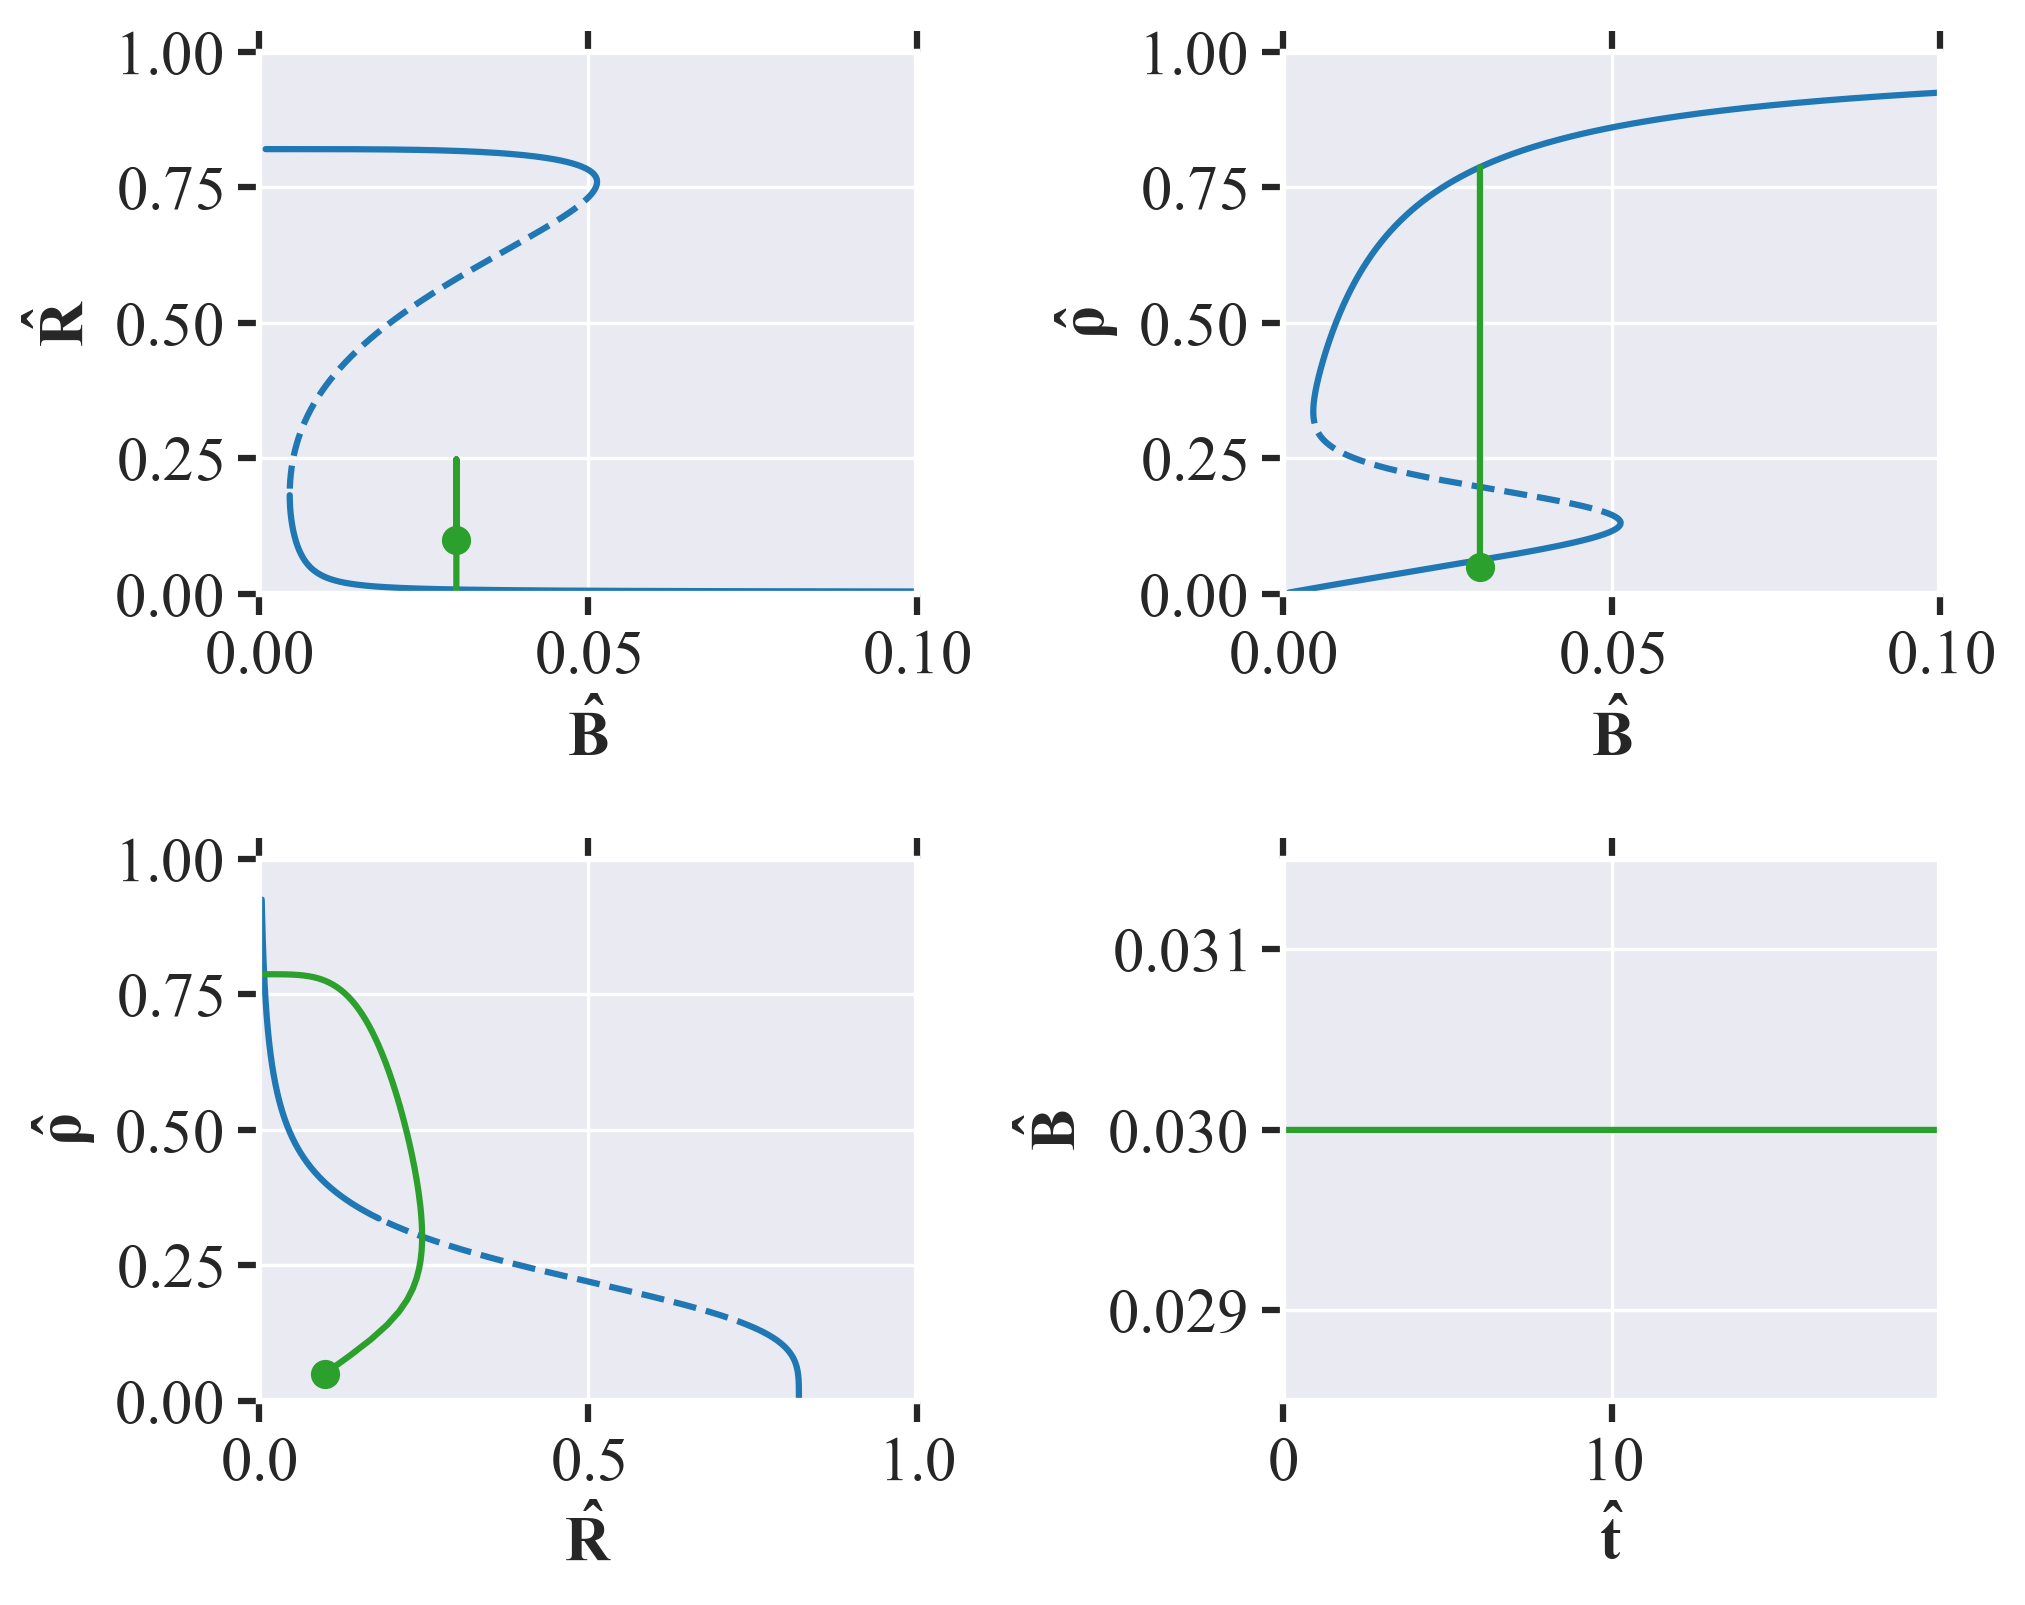
\includegraphics[width= \textwidth]{figures/cell_biology_R0=0.3_rho0=0.16_deltaR=1_n=4_Bmax=0.04_eps=0.0.png}
    \caption{Figure of the continuation of \textbf{top left:} $(\hat{R}, \hat{B})$ and \textbf{top right:}, $(\hat{\rho}, \hat{B})$, \textbf{bottom left:} phase space $(\hat{rho}, \hat{R})$ and 
    \textbf{bottom right:} $\hat{B}$ against time (time horizon of 10 seconds with a timestep of 0.01).}
    \label{fig:cell_biology_ex1}
\end{figure}

\subsection{Conclusion}
\todo{Conclusion to the assignment}